\documentclass[a4paper,oneside,14pt]{extreport}

\usepackage[T2A]{fontenc}
\usepackage[utf8]{inputenc}
\usepackage[english,russian]{babel}

\usepackage[left=30mm, right=10mm, top=20mm, bottom=20mm, bindingoffset=0cm]{geometry}

\usepackage{microtype}
\usepackage{tikz}

\usepackage{setspace}
\onehalfspacing
\usepackage{graphicx}
\usepackage{indentfirst}
\setlength{\parindent}{12.5mm}

\usepackage{titlesec}
\titleformat{\chapter}{\LARGE\bfseries}{\thechapter}{10pt}{\LARGE\bfseries}
\titlespacing*{\chapter}{0pt}{-20pt}{10pt}
\titleformat{\section}{\large\bfseries}{\thesection}{10pt}{\large\bfseries}
\titlespacing*{\section}{0pt}{0pt}{10pt}
\titleformat{\subsection}{\normalsize\bfseries}{\thesubsection}{10pt}{\normalsize\bfseries}
\titlespacing*{\subsection}{0pt}{5pt}{5pt}

\addto{\caption}{\renewcommand*{\contentsname}{Содержание}}
\usepackage[square,sort,comma,numbers]{natbib}
\renewcommand{\bibsection}{\chapter*{Список литературы}}

\usepackage{caption}

\usepackage{wrapfig}
\usepackage{float}
\usepackage{listings}
\usepackage{graphicx}
\graphicspath{{.}}
\newcommand{\imgwc}[4]
{
	\begin{figure}[#1]
		\center{\includegraphics[width=#2]{inc/img/#3}}
		\caption{#4}
		\label{img:#3}
	\end{figure}
}
\newcommand{\imghc}[4]
{
	\begin{figure}[#1]
		\center{\includegraphics[height=#2]{inc/img/#3}}
		\caption{#4}
		\label{img:#3}
	\end{figure}
}
\newcommand{\imgsc}[4]
{
	\begin{figure}[#1]
		\center{\includegraphics[scale=#2]{inc/img/#3}}
		\caption{#4}
		\label{img:#3}
	\end{figure}
}

\usepackage{pgfplots}
\pgfplotsset{compat=newest}

\usepackage{listings}
\usepackage{listingsutf8}
\lstset{
	basicstyle=\footnotesize\ttfamily,
	keywordstyle=\color{blue},
	stringstyle=\color{red},
	commentstyle=\color{gray},
	numbers=left,
	numberstyle=\tiny,
	numbersep=5pt,
	frame=false,
	breaklines=true,
	breakatwhitespace=true,
	inputencoding=utf8/koi8-r
}

\newcommand{\code}[1]{\texttt{#1}}

\usepackage{amsmath}
\usepackage{mathtools}
\usepackage{amssymb}

\usepackage[unicode]{hyperref}
\hypersetup{hidelinks}

\makeatletter
\newcommand{\vhrulefill}[1]
{
	\leavevmode\leaders\hrule\@height#1\hfill \kern\z@
}
\makeatother


\begin{document}
	\pagenumbering{Alph}
\documentclass[../report.tex]{subfiles}
\graphicspath{{\subfix{../images/}}}

\begin{document}
\thispagestyle{empty}
\doublespacing
\noindent
\begin{minipage}[l]{0.15\textwidth}
	\centering
	
\includegraphics{bmstu_low}
\end{minipage}
% нельзя делать пустую строку
\begin{minipage}[r]{0.85\textwidth}
	\centering\bfseries\singlespacing
	Министерство науки и высшего образования Российской Федерации\\
Федеральное государственное бюджетное образовательное учреждение\\
высшего образования\\
«Московский государственный технический университет\\
имени Н.Э. Баумана\\
(национальный исследовательский университет)»\\
(МГТУ им. Н.Э. Баумана)
\end{minipage}

\vspace*{5mm}
\noindent
\rule{\textwidth}{3pt}

\noindent
\MakeUppercase{Факультет}
\underline{«Информатика и системы управления»}

\noindent
\MakeUppercase{Кафедра}
\underline{«Программное обеспечение ЭВМ и информационные технологии»}

\vspace*{4cm}

\noindent
\center{
\textbf{
\MakeUppercase{Отчет\\
о лабораторной работе №5
}\\
\MakeUppercase{Конвеерная обработка данных}\\
по дисциплине:\\
«Анализ алгоритмов»
}}

\vspace*{3cm}

\begin{FlushLeft}
Руководитель: ст. преп. каф. ИУ7 \noindent\underline{\makebox[3em][l]{}} Волкова Л.Л.\\
Исполнитель: студ. гр. ИУ7-55Б \noindent\underline{\makebox[3em][l]{}} Муравьев И.А.
\end{FlushLeft}

\vspace*{\fill}
\center{
Москва 2021
}


\end{document}
\pagenumbering{arabic}
\newpage
\tableofcontents
\lstset{
	language = python,
	basicstyle=\small\sffamily,
	numbers=left,
	numberstyle=\tiny,
	stepnumber=1,
	numbersep=5pt,
	xleftmargin =.19in,
	showspaces=false,
	showstringspaces=false,
	showtabs=false,
	frame=single,
	tabsize=2,
	captionpos=t,
	breaklines=true,
	breakatwhitespace=false,
	escapeinside={\#*}{*)}
}

\newpage

\addcontentsline{toc}{chapter}{Введение}
\chapter*{Введение}

\textbf{Цель:} сравнить классический алгоритм произведения матриц с алгоритмом Копперсмита-Винограда и его оптимизацией.

\textbf{Задачи:}
\begin{enumerate}
	\item Изучить алгоритмы классического произведения матриц и Копперсмита-Винограда.
	\item Реализовать алгоритмы:
	\begin{enumerate}
		\item классического умножения матриц;
		\item Копперсмита-Винограда;
		\item оптимизированный Копперсмита-Винограда.
	\end{enumerate}
	\item Вычислить и сравнить трудоемкость реализуемых алгоритмов на основе выбранной модели вычислений.
	\item Провести сравнительный анализ алгоритмов по затрачиваемым ресурсам (процессорному времени работы).
\end{enumerate}
\newpage

\chapter{ Аналитическая часть}
Умножение матриц - операция, широко применяющаяся в различных программах и приложениях. Использование данной операции повлекло за собой необходимость её программной реализации. Классический алгоритм умножения матриц является интуитивно понятным, поскольку повторяет действия, производимые человеком для нахождения произведения двух матриц. Однако частое использование операции умножения матриц привело к необходимости поиска более быстрой реализации, ведь несмотря на простоту, алгоритмы, основанные на последовательном переборе элементов, для больших объемов данных работают достаточно долго.

Алгоритм Копперсмита-Винограда - это алгоритм умножения квадратных матриц, предложенный в 1987 году Д. Копперсмитом и Ш. Виноградом \cite{CoppersmithAndWinograd}. Изначально ассимптотическая сложность алгоритма составляла $O(n^{2.3755})$, где $n$ - это размер стороны матрицы. Алгоритм Копперсмита-Винограда, с учётом серии улучшений и доработок в последующие годы, обладает лучшей асимптотикой среди известных алгоритмов умножения матриц.

На практике алгоритм Копперсмита — Винограда не используется, поскольку имеет очень большую константу пропорциональности и начинает выигрывать в быстродействии у других известных алгоритмов только для матриц, размер которых превышает память современных компьютеров \cite{RobinsonSara}.
Поэтому пользуются алгоритмом Штрассена по причинам простоты реализации и меньшей константе в оценке трудоемкости \cite{Strassen}.

\section{Классический алгоритм умножения матриц}
Пусть даны две прямоугольные матрицы, причем количество столбцов первой совпадает с количеством строк второй

\begin{equation}
	A_{nm} = \begin{pmatrix}
		a_{11} & a_{12} & \ldots & a_{1m}\\
		a_{21} & a_{22} & \ldots & a_{2m}\\
		\vdots & \vdots & \ddots & \vdots\\
		a_{n1} & a_{n2} & \ldots & a_{nm}
	\end{pmatrix},
	\quad
	B_{mq} = \begin{pmatrix}
		b_{11} & b_{12} & \ldots & b_{1q}\\
		b_{21} & b_{22} & \ldots & b_{2q}\\
		\vdots & \vdots & \ddots & \vdots\\
		b_{m1} & b_{m2} & \ldots & b_{mq}
	\end{pmatrix}
\end{equation}

Тогда матрица $C = A \times B$, называющаяся произведением матриц A и B выглядит следующим образом:

\begin{equation} 
	C_{nq} = \begin{pmatrix}
		c_{11} & c_{12} & \ldots & c_{1q}\\
		c_{21} & c_{22} & \ldots & c_{2q}\\
		\vdots & \vdots & \ddots & \vdots\\
		c_{n1} & c_{n2} & \ldots & c_{nq}
	\end{pmatrix}, 
\end{equation}
где
\begin{equation} \label{eq:classic_multiply}
c_{ij} = \sum_{k=1}^{m}a_{ik}b_{kj}\quad(i=\vec{1, n}, j=\vec{1,q})
\end{equation}

Программная реализация классического алгоритма умножения матриц заключается в прямой реализации формулы \ref{eq:classic_multiply} для вычисления каждого элемента результирующей матрицы.

\section{Алгоритм Копперсмита-Винограда умножения матриц}

Если посмотреть на результат умножения двух матриц, можно заметить, что каждый элемент в нем представляет собой скалярное произведение соответствующих строки и столбца исходных матриц.
Такое умножение допускает предварительную обработку, позволяющую часть работы выполнить заранее.

Рассмотрим два вектора $\vec{u} = (u_1, u_2, u_3, u_4)$ и $\vec{w} = (w_1, w_2, w_3, w_4)$.
Их скалярное произведение равно: $\vec{u} \cdot \vec{w} = u_1 \cdot w_1 + u_2 \cdot w_2 + u_3 \cdot w_3 + u_4 \cdot w_4$, что эквивалентно \ref{eq:vinograd}.
\begin{equation}
\label{eq:vinograd}
\vec{u} \cdot \vec{w} = (u_1 + w_2)(u_2 + w_1) + (u_3 + w_4)(u_4 + w_3) - u_1 \cdot u_2 - u_3 \cdot u_4 - w_1 \cdot w_2 - w_3 \cdot w_4
\end{equation}

Несмотря на то, что второе выражение требует вычисления большего количества операций, чем стандартный алгоритм (вместо четырех умножений вычисляется шесть, вместо трех сложений - десять), выражение в правой части последнего равенства допускает предварительную обработку: его части можно вычислить заранее и запомнить для каждой строки первой матрицы и для каждого столбца второй, что позволит для каждого элемента выполнять лишь два умножения и пять сложений, складывая затем только лишь с двумя предварительно посчитанными суммами соседних элементов текущих строк и столбцов.
Из-за того, что операция сложения быстрее операции умножения в ЭВМ, на практике алгоритм должен работать быстрее стандартного.

\section{Вывод}
Алгоритм Копперсмита-Винограда отличается от классического алгоритма наличием предварительной обработки матриц и уменьшением общего количества операций умножения, которые выполняются медленнее операций сложения.
\newpage
\chapter{Конструкторская часть}
Данный раздел содержит схемы алгоритмов, реализуемых в работе (классический, Копперсмита-Винограда и оптимизированный Копперсмита-Винограда), а также теоретические вычисления трудоемкости для каждого из них.
\section{Схемы алгоритмов}
В данном пункте раздела представлены схемы реализуемых в работе алгоритмов.
\subsection{Схема классического алгоритма}
На рисунке \ref{fig:matmult} представлена схема обычного алгоритма умножения матриц.

\begin{figure}[H]
	\centering
	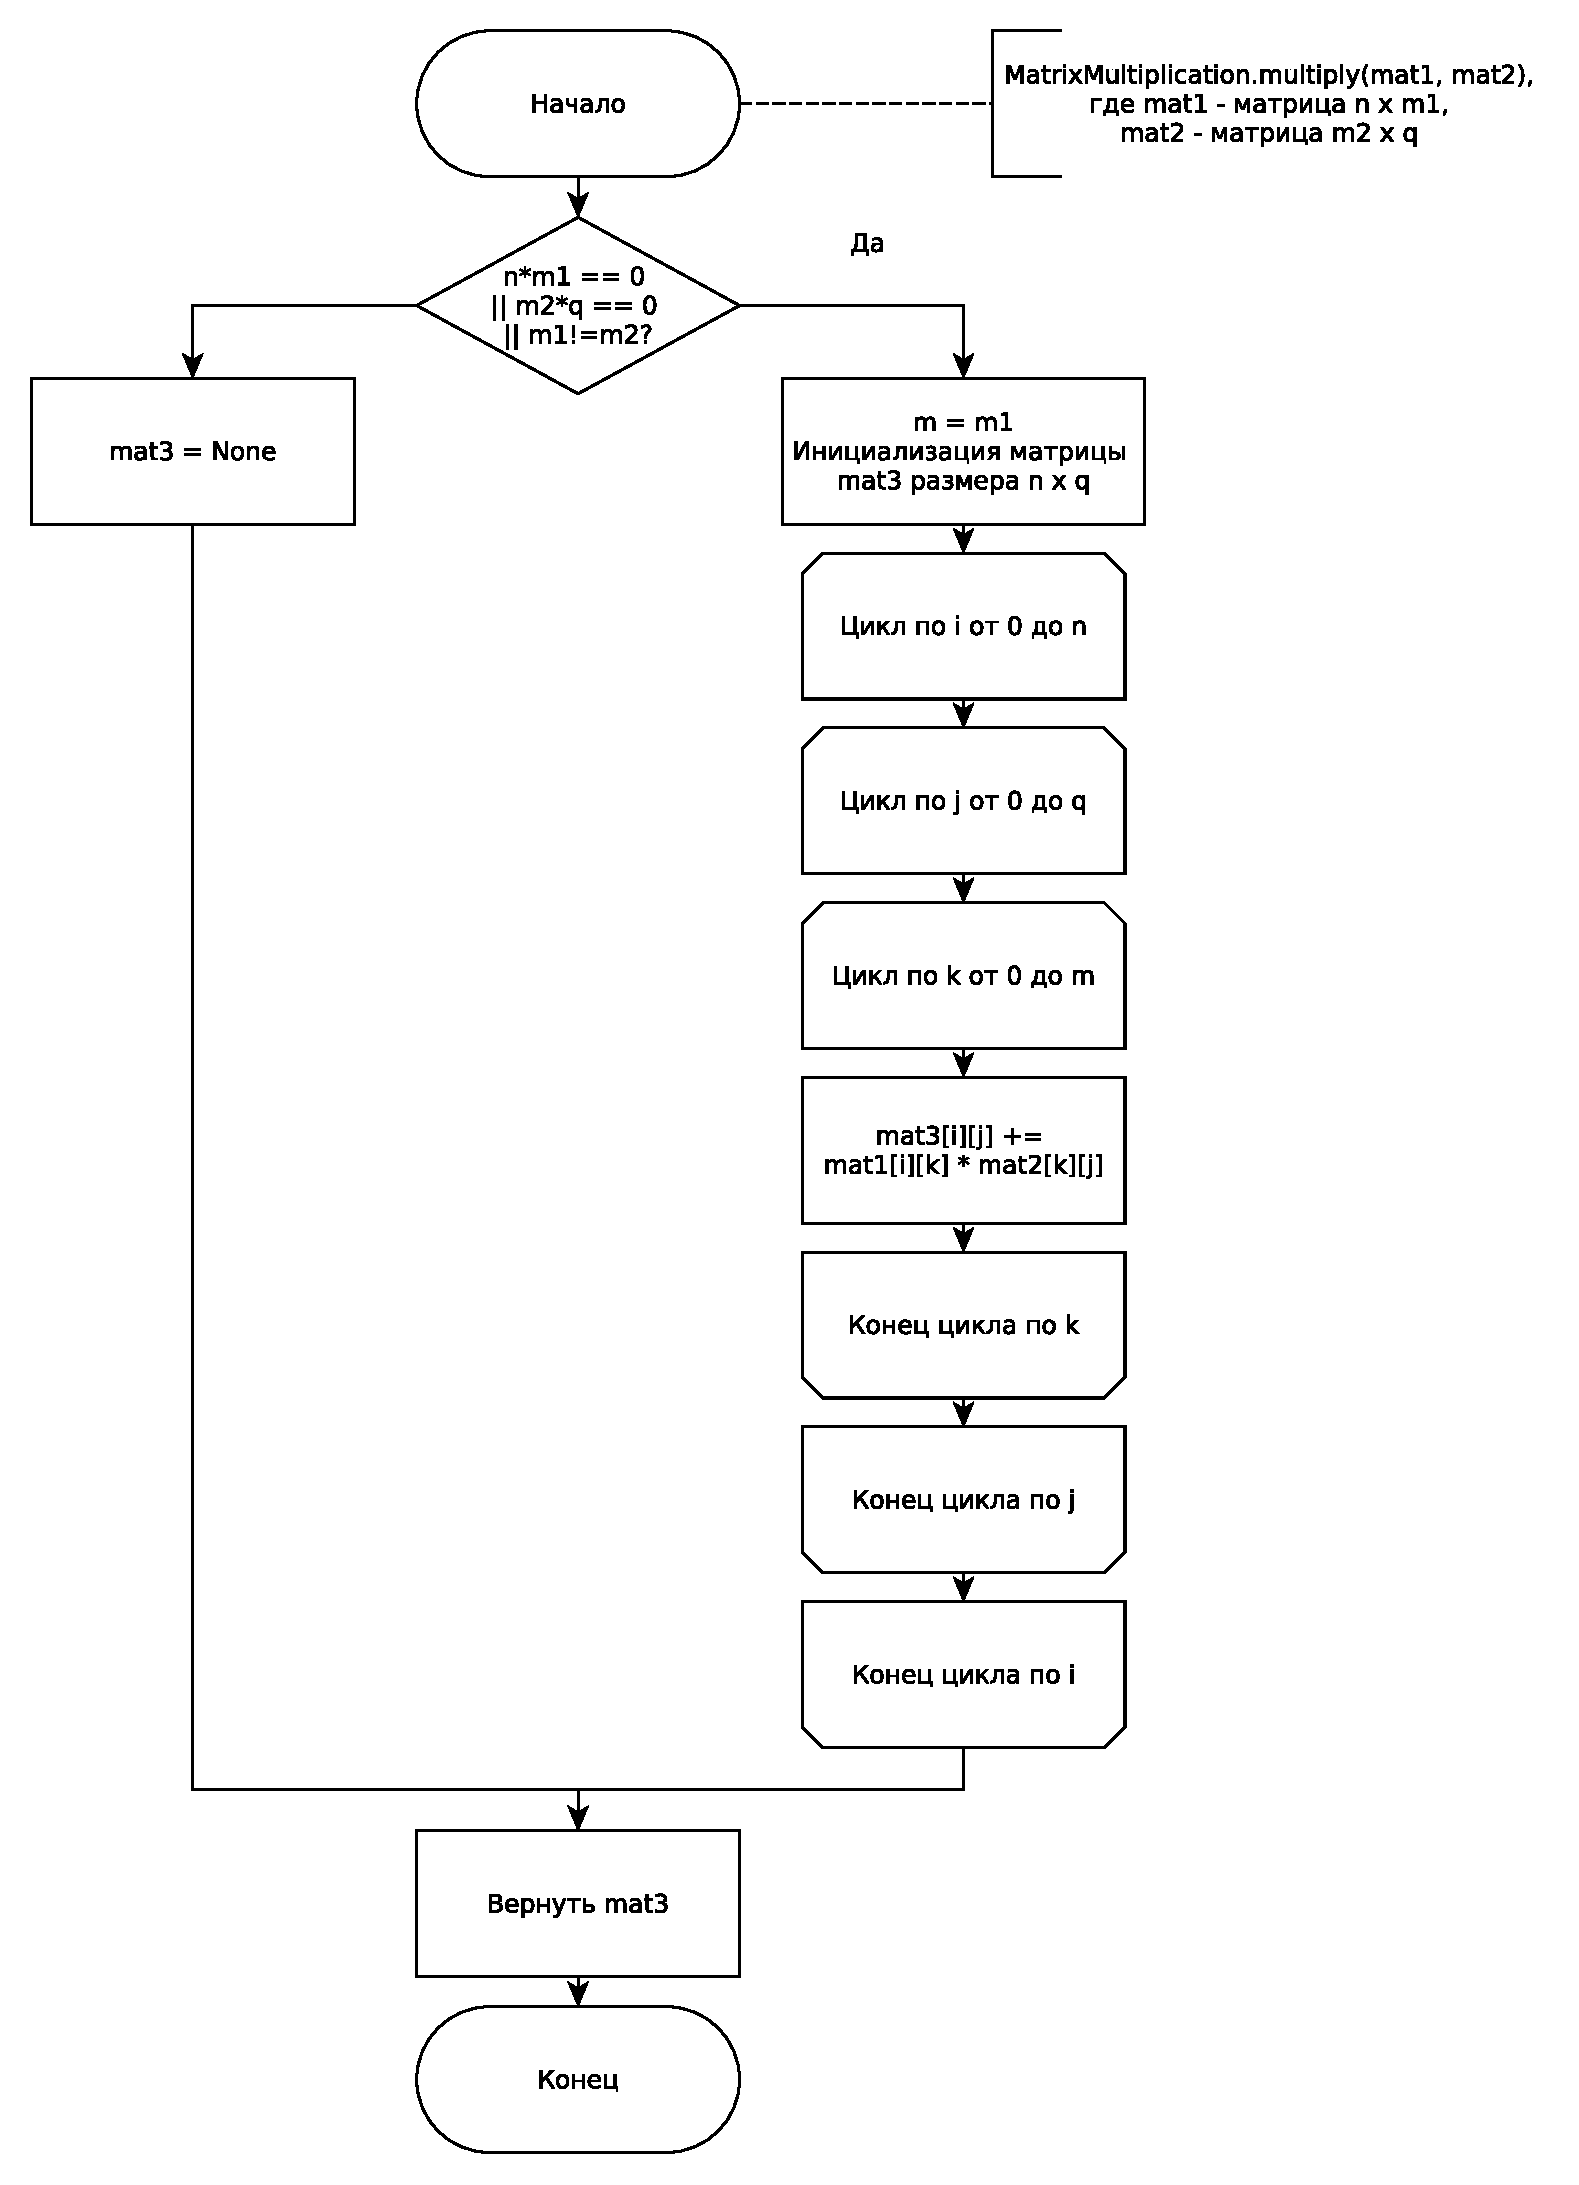
\includegraphics[width=1\linewidth]{images/MatrixMultiplication}
	\caption{Схема стандартного алгоритма умножения матриц}
	\label{fig:matmult}
\end{figure}

\subsection{Схема алгоритма Копперсмита-Винограда}
На рисунках \ref{fig:vin_mulh}-\ref{fig:vinograd} представлены схемы алгоритма Копперсмита-Винограда умножения матриц.

\captionsetup{justification=centering, singlelinecheck=false}

\begin{figure}[H]
	\centering
	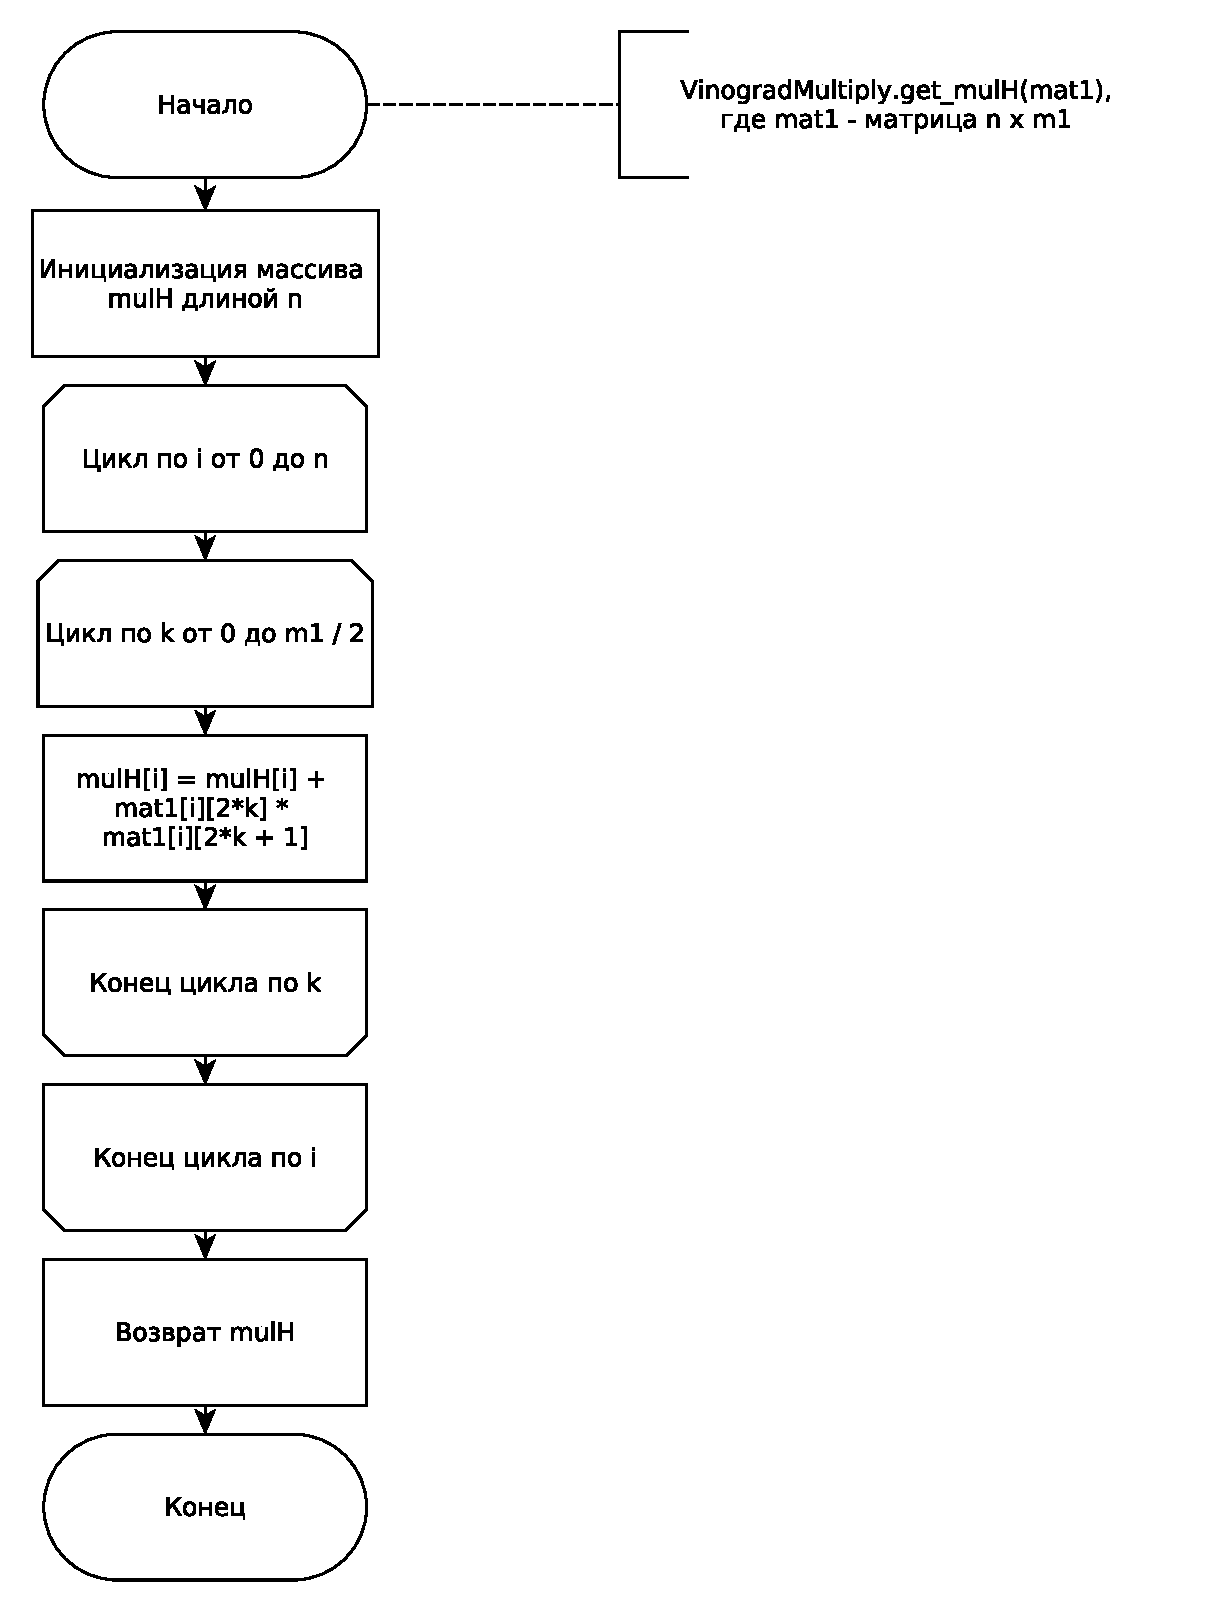
\includegraphics[width=0.9\linewidth]{images/vinograd_get_mulh}
	\caption{Схема функции предварительной обработки первой матрицы для алгоритма Винограда}
	\label{fig:vin_mulh}
\end{figure}

\begin{figure}[H]
	\centering
	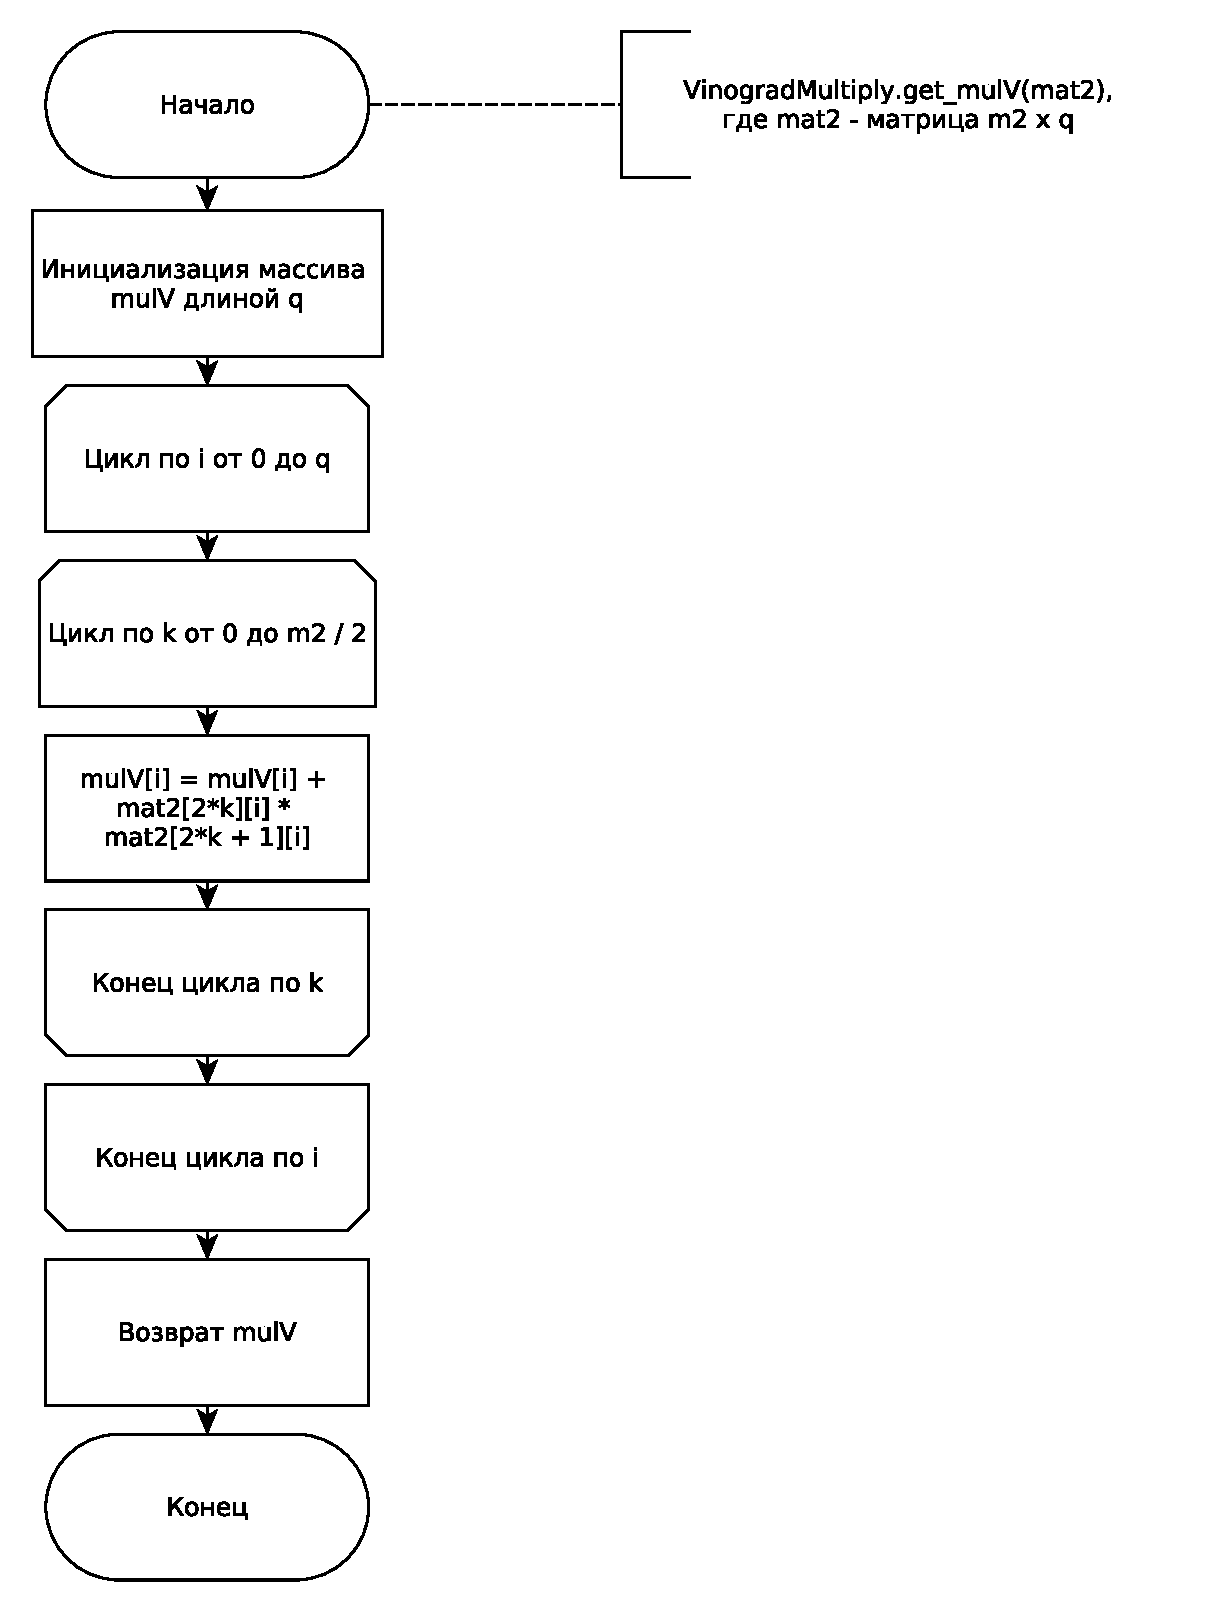
\includegraphics[width=0.9\linewidth]{images/vinograd_get_mulv}
	\caption{Схема функции предварительной обработки второй матрицы для алгоритма Винограда}
	\label{fig:vin_mulv}
\end{figure}

\begin{figure}[H]
%\centering
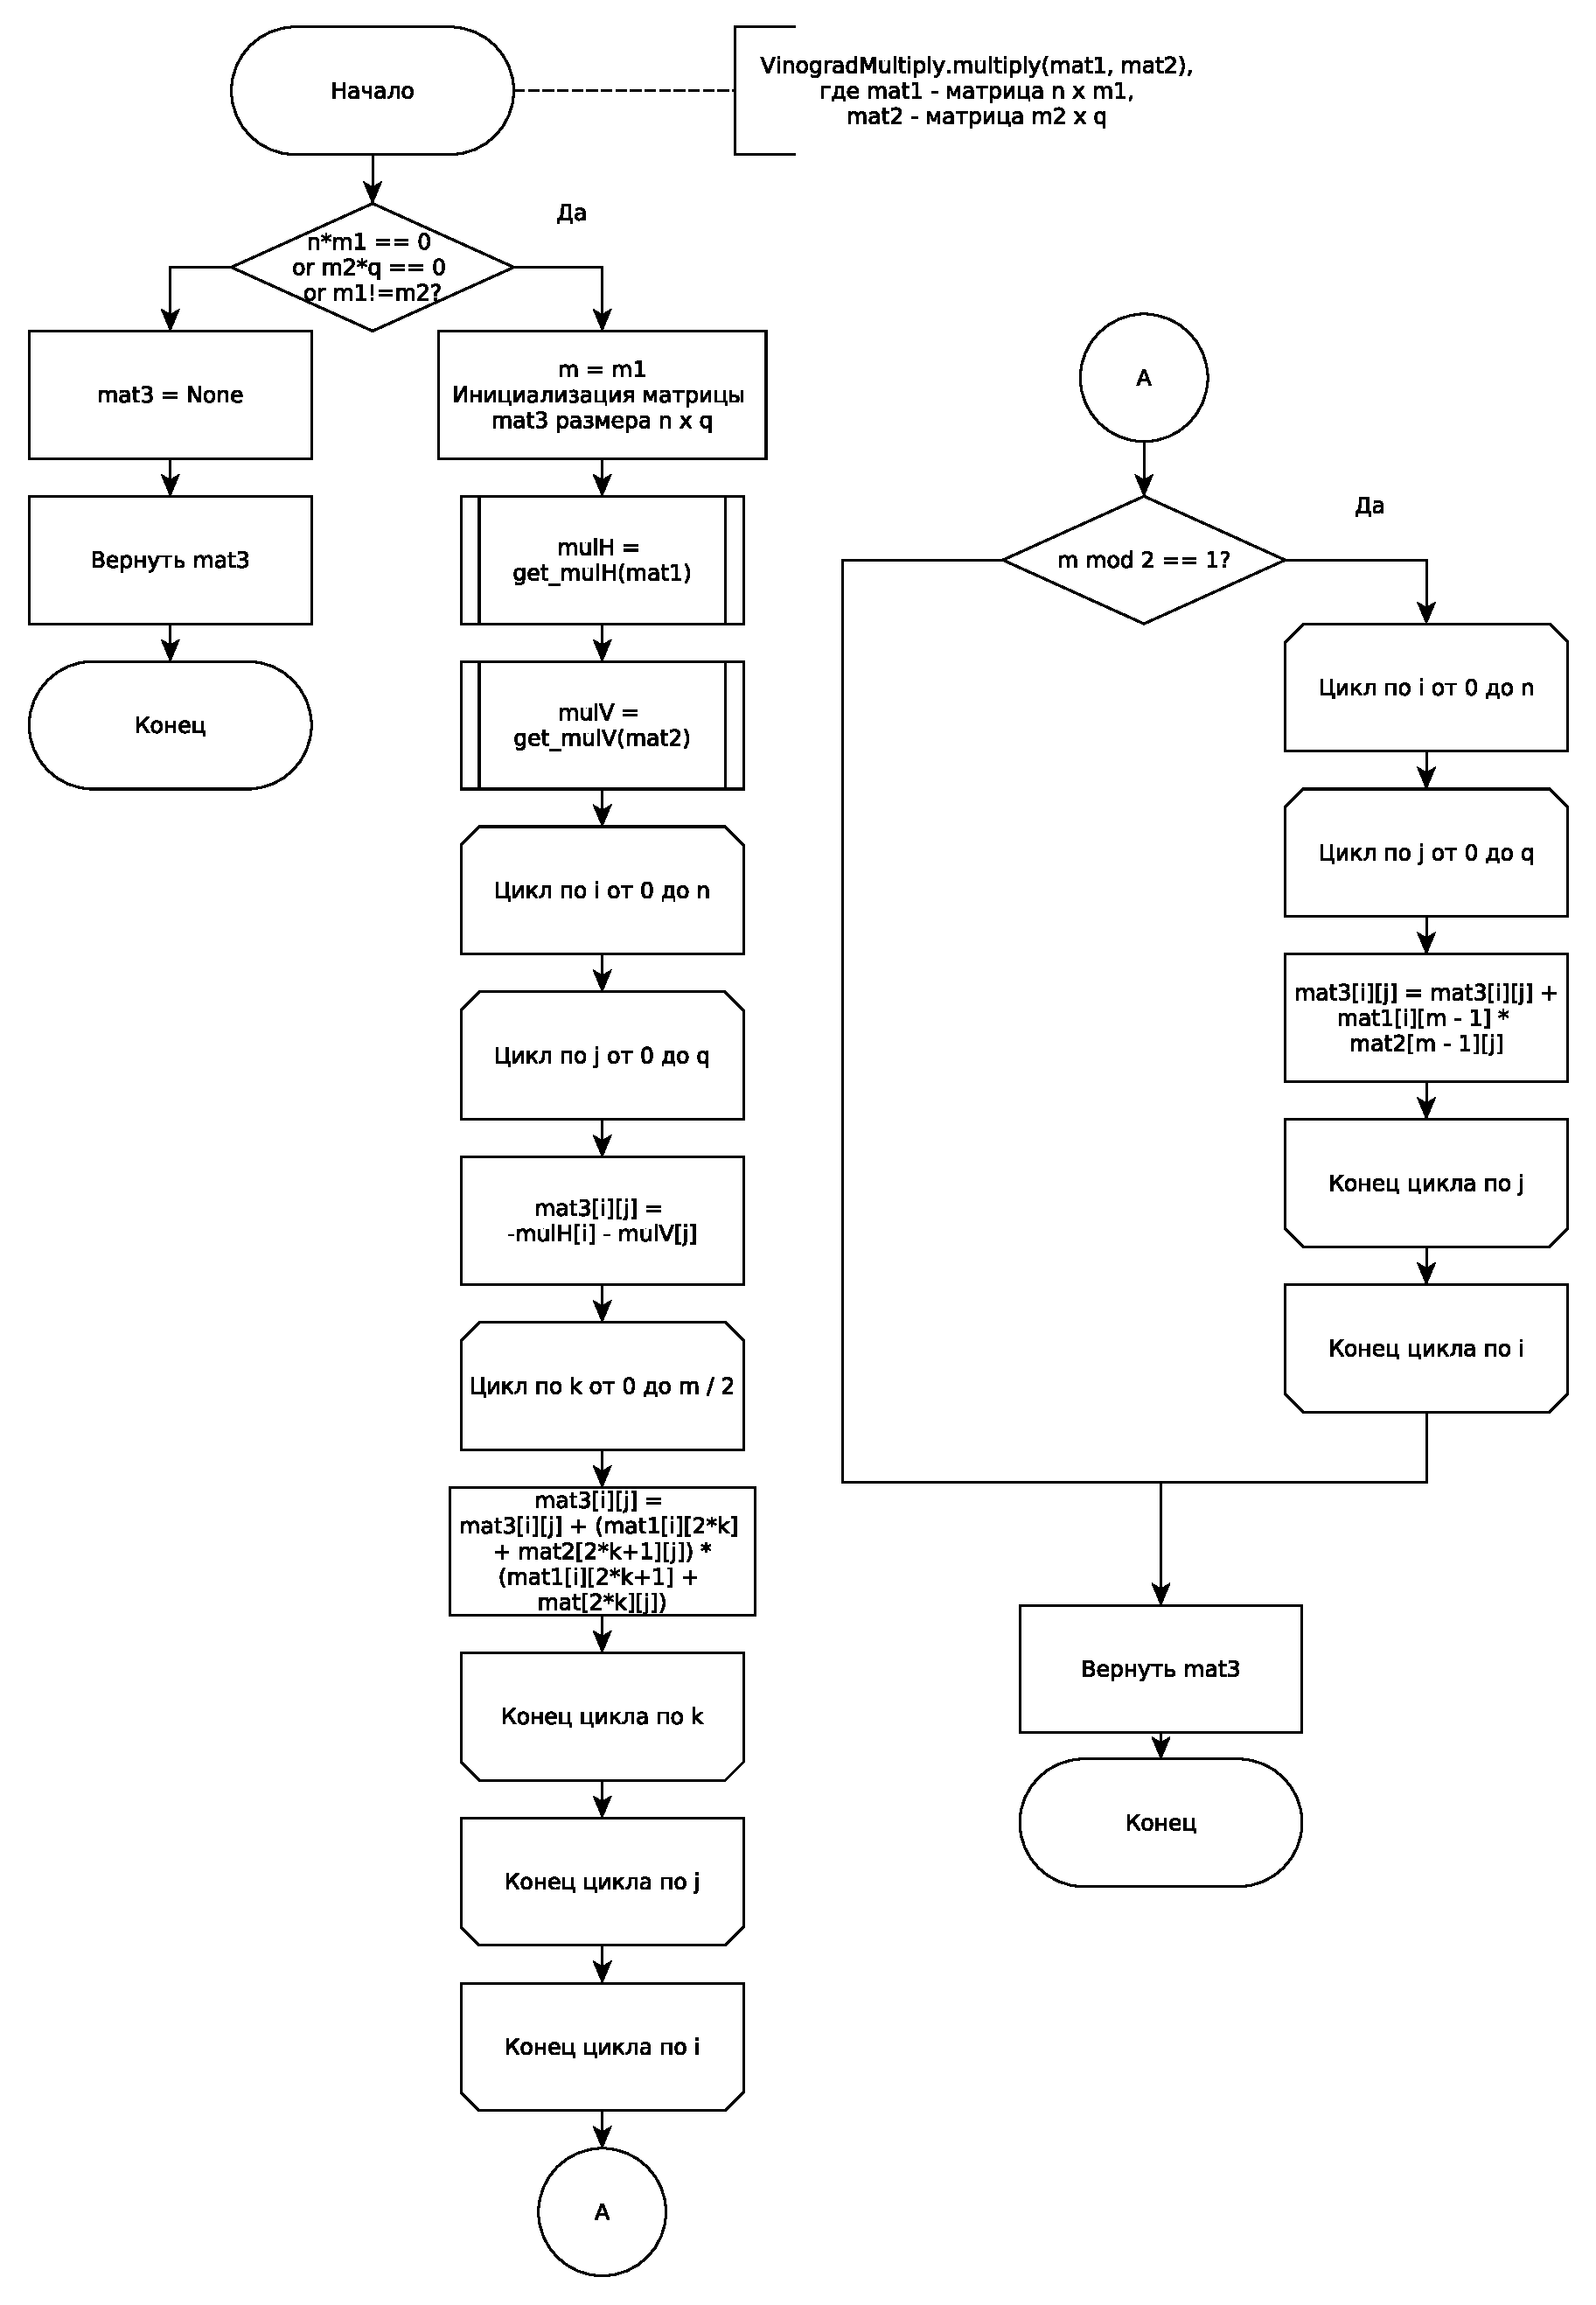
\includegraphics[width=1\linewidth]{images/vinograd}
\caption{Схема алгоритма Винограда}
\label{fig:vinograd}
\end{figure}


\subsection{Схема оптимизированного алгоритма Копперсмита-Винограда}
Оптимизации алгоритма Копперсмита-Винограда, используемые в улучшенном варианте:
\begin{itemize}
	\item замена двух операций $a = a + \ldots$ на одну a~$+= \ldots$;
	\item замена циклов до $n/2$ на циклы до n-1 с шагом 2;
	\item сокращение затрат на получение значения по индексам за счет ввода аккумулирующей промежуточное значение переменной buff;
	\item соединение двух циклов и сокращение затрат на содержание второго идентичного цикла для матриц нечетных размерностей.
\end{itemize}

Схема улучшенного алгоритма представлена на рисунках \ref{fig:opt_vin_mulh} - \ref{fig:opt_vinograd}.


\begin{figure}[H]
	\centering
	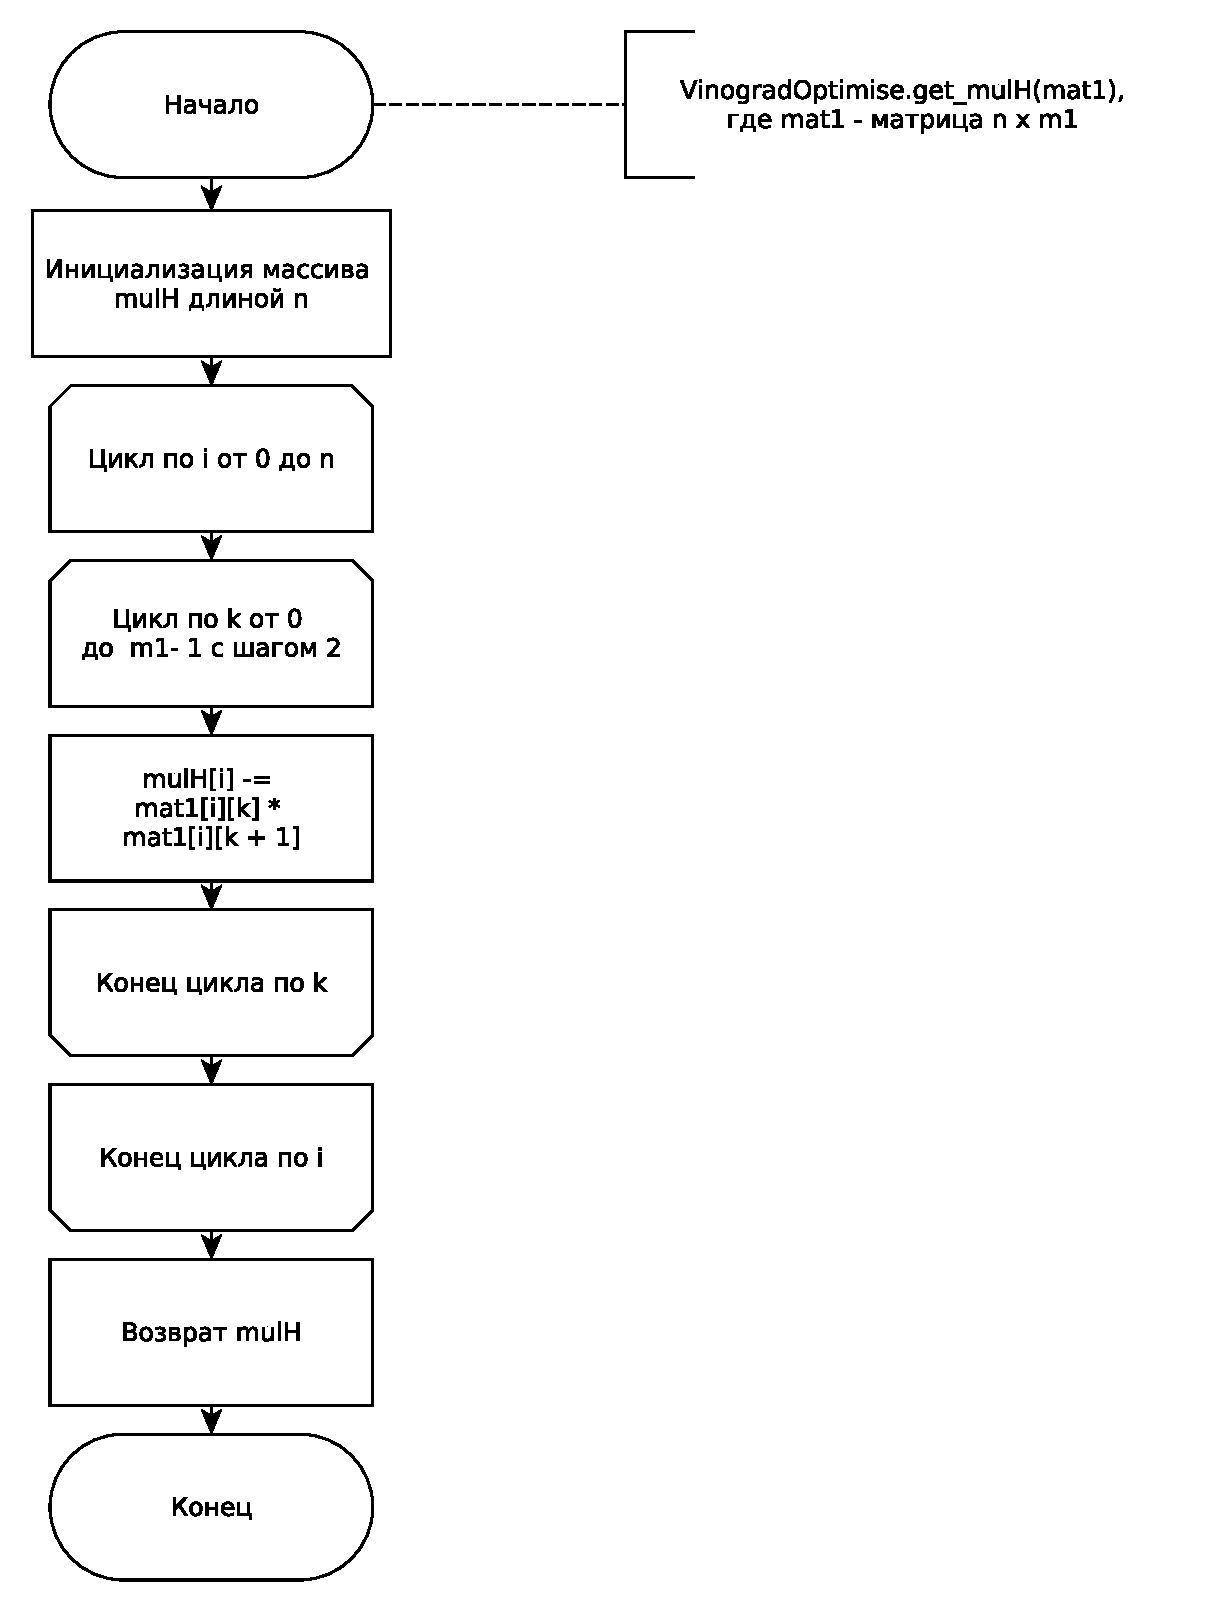
\includegraphics[width=0.9\linewidth]{images/vinogradOptimise_get_mulh}
	\caption{Схема функции предварительной обработки первой матрицы для оптимизированного алгоритма Винограда}
	\label{fig:opt_vin_mulh}
\end{figure}

\begin{figure}[H]
	\centering
	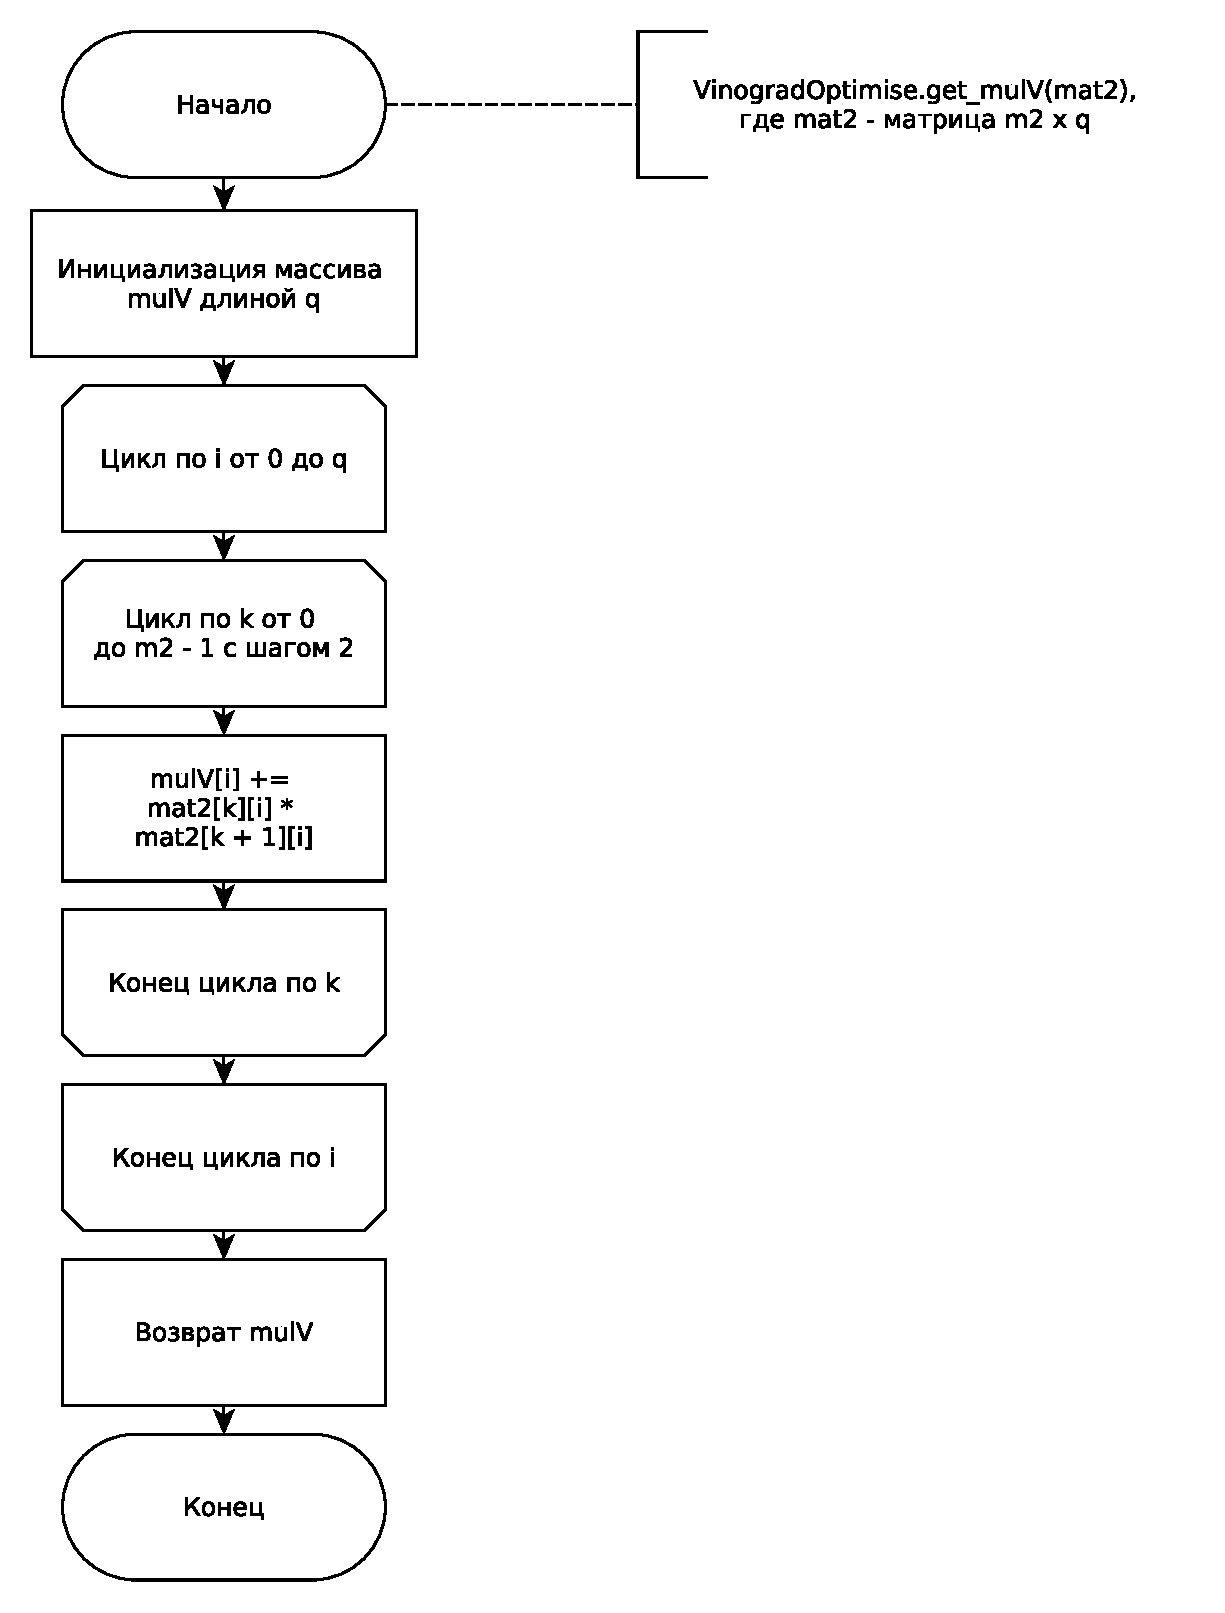
\includegraphics[width=0.9\linewidth]{images/vinogradOptimise_get_mulv}
	\caption{Схема функции предварительной обработки второй матрицы для оптимизированного алгоритма Винограда}
	\label{fig:opt_vin_mulv}
\end{figure}

\begin{figure}[H]
	%\centering
	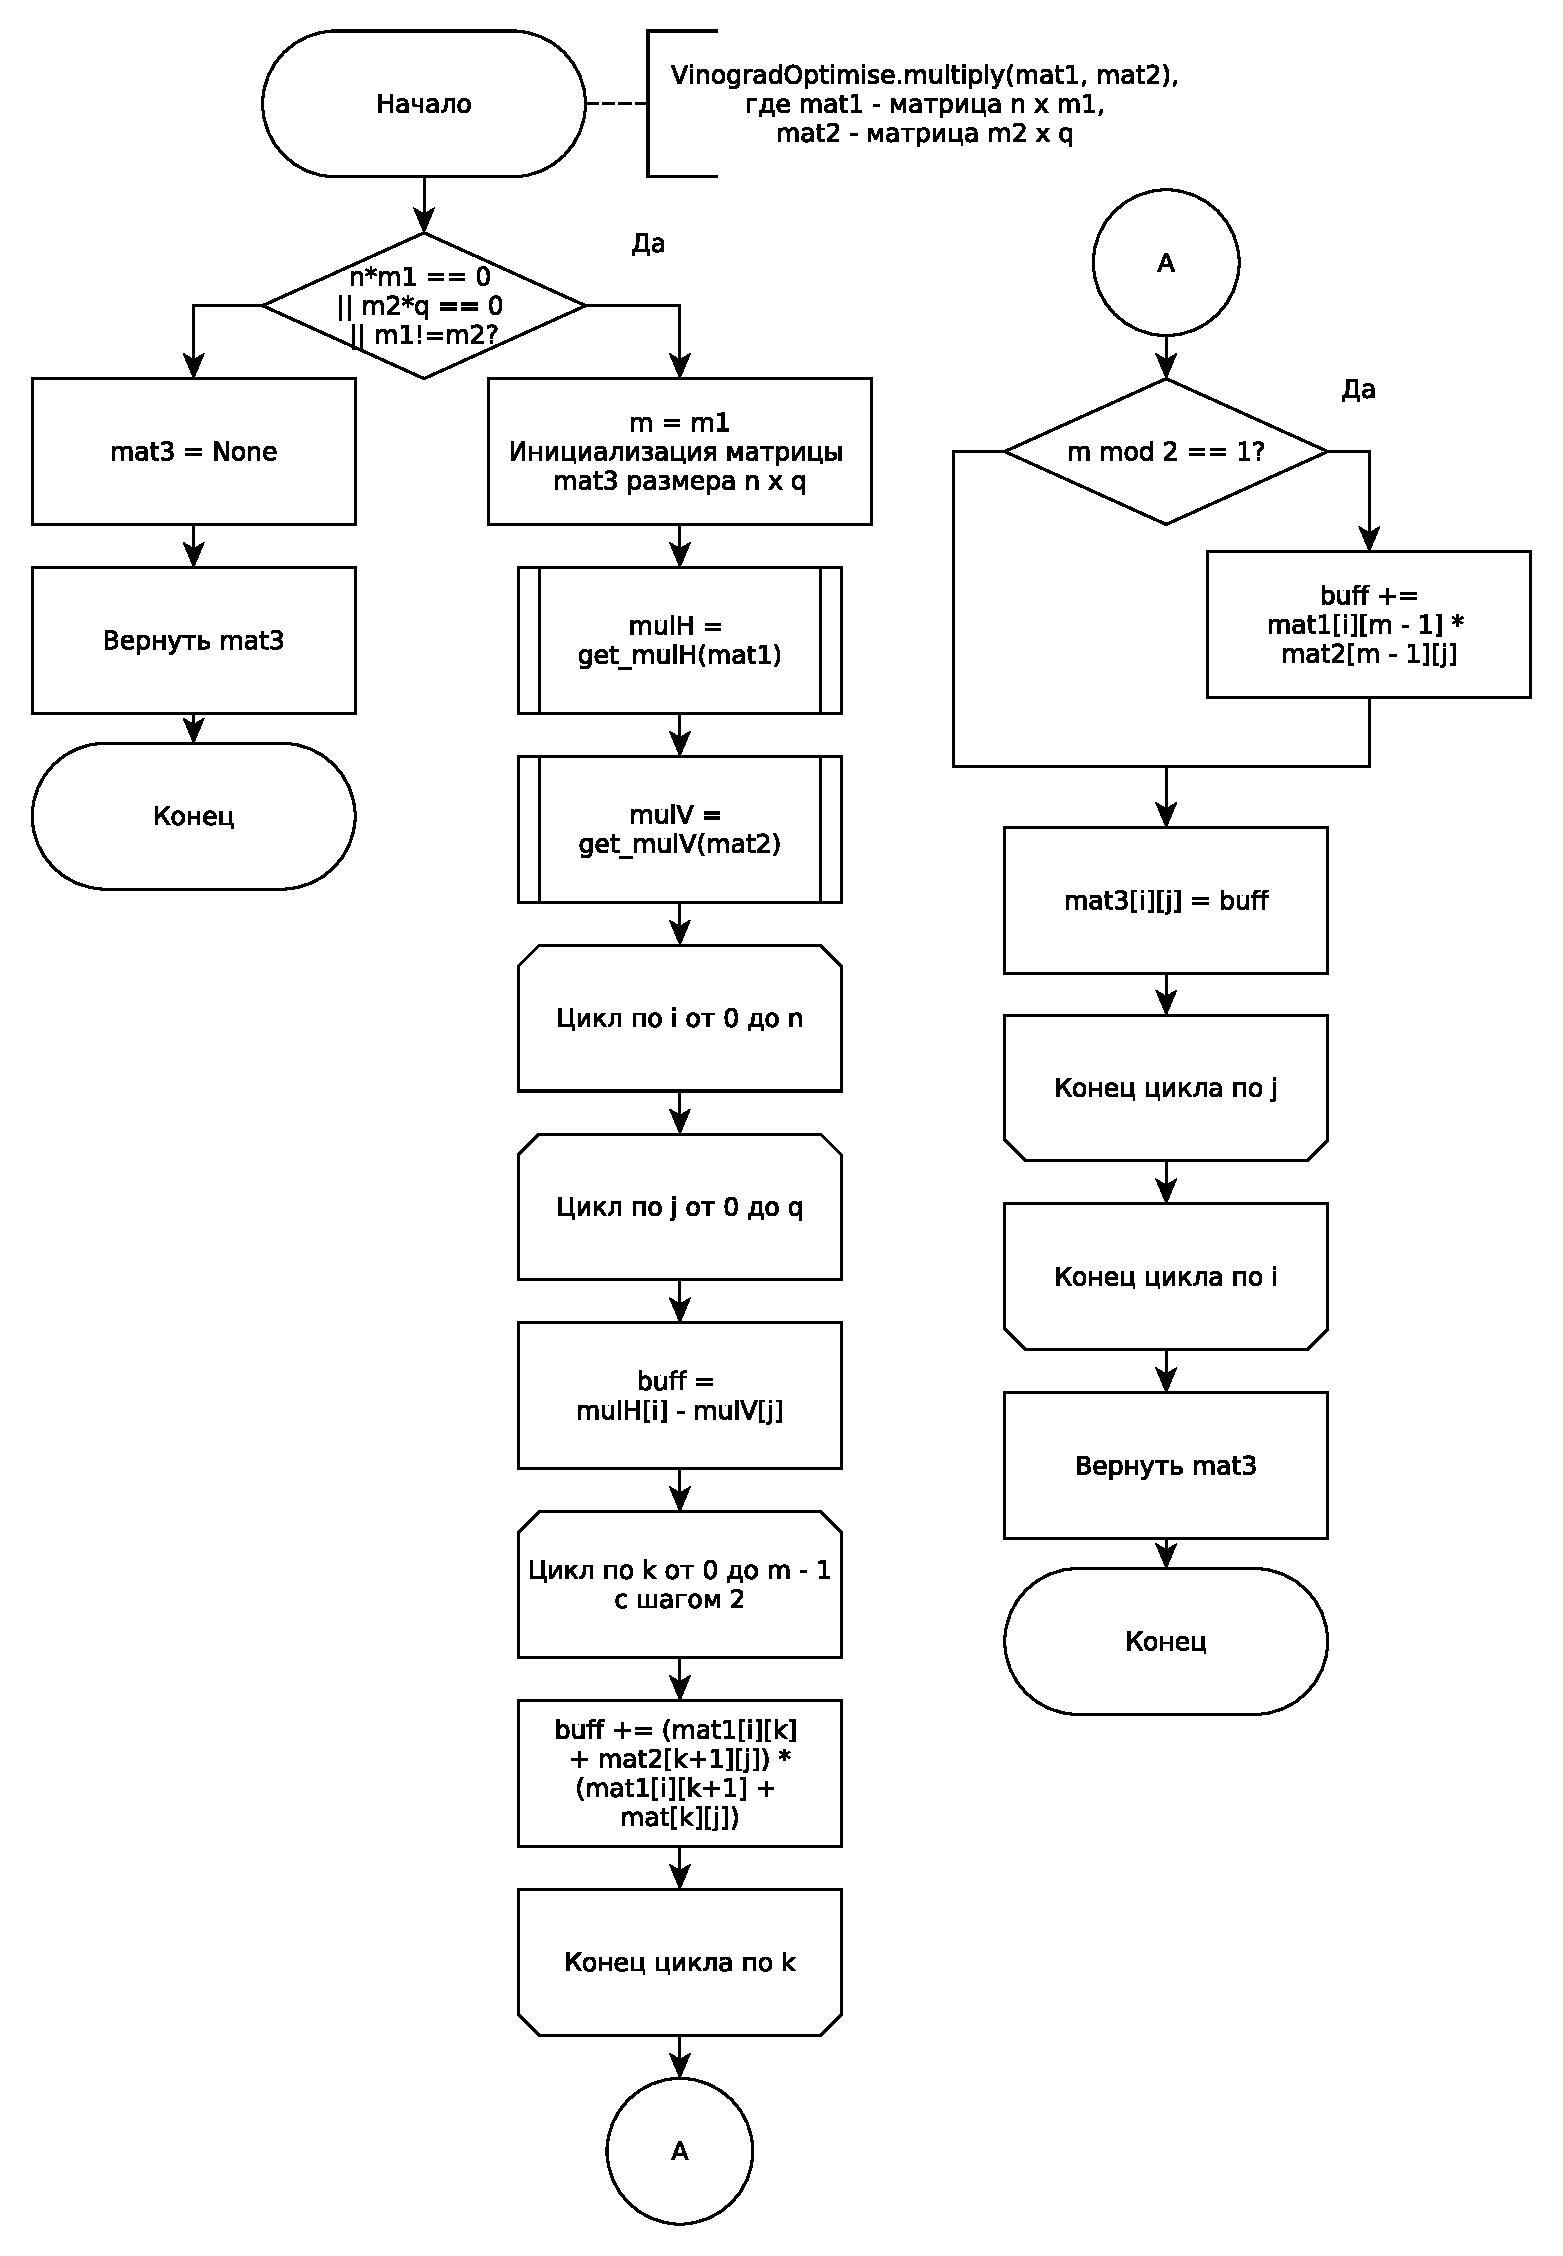
\includegraphics[width=1\linewidth]{images/VinogradOptimise}
	\caption{Схема оптимизированного алгоритма Винограда}
	\label{fig:opt_vinograd}
\end{figure}

\section{Модель вычислений}

В данной работе используется следующая модель вычислений для определения трудоемкости алгоритмов:
\begin{itemize}
	\item операции из списка \ref{eq:op_1} имеют трудоемкость 1;
	\begin{equation} \label{eq:op_1}
	+, -, +=, -=, =, ==, !=, !, \&\&, ||, <, >, <<, >>, <=, >=, [] 
	\end{equation}
	\item операции из списка \ref{eq:op_2} имеют трудоемкость 2;
	\begin{equation} \label{eq:op_2}
	*, /, //, \%, *=, /=
	\end{equation}
	\item трудоемкость цикла рассчитывается по формуле \ref{eq:for};
	\begin{equation} \label{eq:for}
	\begin{array}{ll}
		f_{\text{цикла for}} = f_{\text{инициализации}} + f_{\text{сравнения}} +\\
		N_{\text{итераций}} (f_{\text{тела}} + f_{\text{инкремента}} + f_{\text{сравнения}})
	\end{array}
	\end{equation}
	\item трудоемкость условного оператора if ($
	\begin{array}{ll}
	if (\text{условие}) \ then \ \{A\}\ else \	 \{B\}  
	\end{array}
	$) рассчитывается по формуле \ref{eq:if_cnt} с учетом того, что трудоемкость условного перехода равна 0. \\
	\begin{equation} \label{eq:if_cnt}
	f_{if} = f_{\text{условия}} +
	\begin{cases}
	min(f_A, f_B), & \textrm{лучший случай}\\
	max(f_A, f_B), & \textrm{худший случай}
	\end{cases}
	\end{equation}
\end{itemize}

\section{Трудоемкость алгоритмов умножения матриц}
В данном подразделе представлены расчеты трудоемкости для алгоритмов за исключением затрат на проверку корректности входных данных и инициализацию результирующей матрицы.
\subsection{Трудоемкость классического алгоритма}
Трудоемкость классического алгоритма умножения матриц складывается из следующих частей:
\begin{itemize}
	\item внешний цикл от 0 до n: $f_{for i}=1 + 1 + n(1 + 1 + f_{\text{тела i}}) = 2 + n(2 + f_{\text{тела i}})$;
	\item вложенный цикл от 0 до q: $f_{for_j}=1 + 1 +q(1 + 1 + f_{\text{тела j}}) = 2 + q(2 + f_{\text{тела j}})$;
	\item внутренний цикл от 0 до m: $f_{for_k}=1 + 1 + m(1 + 1 + f_{\text{тела k}}) = 2 + m(2 + f_{\text{тела k}})$;
	\item Тело внутреннего цикла: $f_{\text{тела k}} = 1 \cdot 6 + 1 + 2 = 9$.
\end{itemize}

Подставив вложенные циклы как тела внешних по отношению к ним, вычислим общую трудоемкость алгоритма, представленную в формуле \ref{eq:classic_cnt}.
\begin{equation} \label{eq:classic_cnt}
\begin{array}{ll}
f_{\text{классический}} = 2 + n(2 + 2 + q(2 + 2 + m(2 + 9))) =\\
11mnq + 4nq + 4n + 2 \approx 11mnq
\end{array}
\end{equation}

\subsection{Трудоемкость алгоритма Копперсмита-Винограда}
Трудоемкость алгоритма Винограда умножения матриц содержит следующие части:
\begin{itemize}
	\item создание и инициализация массива mulH:
	\begin{itemize}
		\item цикл от 0 до n: $f_{for_i}=1 + 1 + n(1 + 1 + f_{\text{тела i}}) = 2 + n(2 + f_{\text{тела i}})$;
		\item цикл от 0 до m/2: $f_{for_k}=1 + 1 + 2 + \frac{m}{2}(1 + 1 + 2 + f_{\text{тела k}}) = 4 + \frac{m}{2}(4 + f_{\text{тела k}})$;
		\item тело внутреннего цикла: $f_{\text{тела k}} = 1 \cdot 6 + 1 + 1\cdot2 + 3 \cdot 2 = 15$;
	\end{itemize}
	\item создание и инициализация массива mulV:
	\begin{itemize}
		\item цикл от 0 до n: $f_{for_i}=1 + 1 + q(1 + 1 + f_{\text{тела i}}) = 2 + q(2 + f_{\text{тела i}})$;
		\item цикл от 0 до m/2: $f_{for_k}=1 + 1 + 2 + \frac{m}{2}(1 + 1 + 2 + f_{\text{тела k}}) = 4 + \frac{m}{2}(4 + f_{\text{тела k}})$;
		\item тело внутреннего цикла: $f_{\text{тела k}} = 1 \cdot 6 + 1 + 1\cdot2 + 3 \cdot 2 = 15$;
	\end{itemize}
	\item заполнение матрицы:
	\begin{itemize}
		\item цикл от 0 до n: $f_{for_i}=1 + 1 + n(1 + 1 + f_{\text{тела i}}) = 2 + n(2 + f_{\text{тела i}})$;
		\item вложенный цикл от 0 до q: $f_{for_j}=1 + 1 +q(1 + 1 +	1 \cdot 4 + 1 + 1 \cdot 2 + f_{for_k}) = 2 + q(9 + f_{for_k})$;
		\item внутренний цикл от 0 до m/2: $f_{for_k}=1 + 1 + 2 + \frac{m}{2}(1 + 1 + 2 + f_{\text{тела k}}) = 4 + \frac{m}{2}(4 + f_{\text{тела k}})$;
		\item тело внутреннего цикла: $f_{\text{тела k}} = 1 \cdot 12 + 1 + 1 \cdot 5 + 5 \cdot 2 = 28$;
		\item проверка нечетности размера: $f_{check} = 3$;
	\item цикл для дополнения умножения суммой последних нечетных строки и столбца, если общий размер нечетный (худший случай):
	\begin{itemize}
		\item цикл  от 0 до n: $f_{for_i}=1 + 1 + n(1 + 1 + f_{\text{тела i}}) = 2 + n(2 + f_{\text{тела i}})$;
		\item цикл от 0 до q: $f_{for_j}=1 + 1 +q(1 + 1 + f_{\text{тела j}}) = 2 + q(2 + f_{\text{тела j}})$;
		\item тело внутреннего цикла: $f_{\text{тела j}} = 1 \cdot 8 + 1 + 1 + 1 \cdot 2 + 2  = 14$.
	\end{itemize}
	
	\end{itemize}
\end{itemize}

Таким образом, для лучшего случая получим выражение \ref{eq:vinograd_best_case}.
\begin{equation} \label{eq:vinograd_best_case}
\begin{array}{ll}
f = 2 + n(2 + 4 + \frac{m}{2}(4 + 15)) + 2 + q(2 + 4 + \frac{m}{2}(4 + 15)) + 2 + \\
n(2 + 2 + q(9 + 4 + \frac{m}{2}(4 + 28))) + 3 = \\
16mnq + 13nq + \frac{19}{2}mn + \frac{19}{2}mq + 10n + 6q + 9 \approx 16 mnq
\end{array}
\end{equation}

Для худшего случая получим выражение \ref{eq:vinograd_worst_case}.
\begin{equation} \label{eq:vinograd_worst_case}
\begin{array}{ll}
f = 2 + n(2 + 4 + \frac{m}{2}(4 + 15)) + 2 + q(2 + 4 + \frac{m}{2}(4 + 15)) + 2 + \\
n(2 + 2 + q(9 + 4 + \frac{m}{2}(4 + 28))) + 3 + 2 + n(2 + 2 + q(2 + 14))= \\ 16mnq + 29nq + \frac{19}{2}mn + \frac{19}{2}mq + 14n + 6q + 11 \approx 16 mnq
\end{array}
\end{equation}

\subsection{Трудоемкость оптимизированного алгоритма Копперсмита-Винограда}
Трудоемкость оптимизированного алгоритма Винограда умножения матриц включает в себя следующие составляющие:
\begin{itemize}
	\item создание и инициализация массива mulH:
	\begin{itemize}
		\item цикл от 0 до n: $f_{for_i}=1 + 1 + n(1 + 1 + f_{\text{тела i}}) = 2 + n(2 + f_{\text{тела i}})$;
		\item цикл от 0 до m - 1 с шагом 2: $f_{for_k}=1 + 1 + 1 + \frac{m-1}{2}(1 + 1 + 1 + f_{\text{тела k}}) = 3 + \frac{m-1}{2}(3 + f_{\text{тела k}})$;
		\item тело внутреннего цикла: $f_{\text{тела k}} = 1 \cdot 5 + 1 + 2 + 1 = 9$;
	\end{itemize}
	\item создание и инициализация массива mulV:
	\begin{itemize}
		\item цикл от 0 до n: $f_{for_i}=1 + 1 + q(1 + 1 + f_{\text{тела i}}) = 2 + q(2 + f_{\text{тела i}})$;
		\item цикл от 0 до m-1 с шагом 2: $f_{for_k}=1 + 1 + 1 + \frac{m-1}{2}(1 + 1 + 1 + f_{\text{тела k}}) = 3 + \frac{m-1}{2}(3 + f_{\text{тела k}})$;
		\item тело внутреннего цикла: $f_{\text{тела k}} = 1 \cdot 5 + 1 + 2 + 1 = 9$;
	\end{itemize}
	\item заполнение матрицы:
	\begin{itemize}
		\item цикл от 0 до n: $f_{for_i}=1 + 1 + n(1 + 1 + f_{\text{тела i}}) = 2 + n(2 + f_{\text{тела i}})$;
		\item вложенный цикл от 0 до q: $f_{for_j}=1 + 1 +q(1 + 1 + 1 + 2\cdot1 + 1 + f_{for_k}) = 2 + q(6 + f_{for_k} + f_{check} + f_{add} + f_{rem})$;
		\item внутренний цикл от 0 до m-1 с шагом 2: $f_{for_k}=1 + 1 + 1 + \frac{m-1}{2}(1 + 1 + 1 + f_{\text{тела k}}) = 3 + \frac{m-1}{2}(3 + f_{\text{тела k}})$;
		\item тело внутреннего цикла: $f_{\text{тела k}} = 1 \cdot 8 + 1 + 4 + 2 = 15$;
		\item проверка нечетности размера: $f_{check} = 3$;
		\item дополнение умножения суммой последних нечетных строки и столбца, если общий размер нечетный (худший случай): $f_{\text{add}} = 1 \cdot 4 + 1 + 1\cdot2 + 2 = 9$;
		\item запоминание промежуточного значения: $f_{rem} = 1\cdot2+1 = 3$.
	\end{itemize}
\end{itemize}

Основываясь на приведенных выше выражениях, трудоемкость лучшего случая оптимизированного алгоритма Копперсмита-Винограда выразим формулой \ref{eq:optimised_best_case}.
\begin{equation} \label{eq:optimised_best_case}
\begin{array}{ll}
f = 2 + n(2 + 3 + \frac{m-1}{2}(3 + 9)) + 2 + q(2 + 3 + \frac{m-1}{2}(3 + 9)) + 2 + \\
n(2 + 2 + q(6 + 3 + \frac{m-1}{2}(3 + 15) + 3 + 3)) =\\
 9mnq + 6nq + 6mq + 6mn+3n-q+6 \approx 9mnq
\end{array}
\end{equation}

Трудоемкость худшего случая вычисляется по формуле \ref{eq:optimised_worst_case}.
\begin{equation} \label{eq:optimised_worst_case}
\begin{array}{ll}
f = 2 + n(2 + 3 + \frac{m-1}{2}(3 + 9)) + 2 + q(2 + 3 + \frac{m-1}{2}(3 + 9)) + 2 + \\
n(2 + 2 + q(6 + 3 + \frac{m-1}{2}(3 + 15) + 3 + 3 + 9)) = \\
9mnq+15nq+6mq+6mn+3n-q+6\approx 9mnq
\end{array}
\end{equation}


\section{Вывод}
В данном разделе на основе приведенных в аналитическом разделе теоретических данных были составлены схемы алгоритмов для реализации в технологической части, вычислена трудоемкость лучшего и худшего случаев алгоритмов. Приблизительная трудоемкость классического алгоритма умножения матриц равна $11mnq$, алгоритма Копперсмита-Винограда - $16mnq$, оптимизированного алгоритма Копперсмита-Винограда - $9mnq$.
\newpage

\chapter{Технологическая часть}
Данный раздел содержит обоснование выбора языка и среды разработки, реализацию алгоритмов.

\section{Требования к программному обеспечению}
Требования, выдвигаемые к разрабатываемому ПО:
\begin{itemize}
	\item входные данные - размеры двух матриц, их элементы;
	\item выходные данные - матрица, являющаяся произведением первой входной матрицы на вторую.
\end{itemize}

\section{Средства реализации}
Для реализации программы был выбран язык программирования Python~\cite{python}. Такой выбор обусловлен следующими причинами:
\begin{itemize}
	\item имеется большой опыт разработки;
	\item имеет большое количество расширений и библиотек, что облегчает работу с некоторыми типами данных и математическими формулами;
	\item обладает информативной документацией.
\end{itemize}

\section{Реализация алгоритмов}
В листингах \ref{lst:classic} - \ref{lst:optVinograd} представлены реализации рассматриваемых алгоритмов.
\newpage
\captionsetup{singlelinecheck=false}
\begin{lstlisting}[caption=Классический алгоритм, label={lst:classic}]
class MatrixMultiplication:
	def __init__(self):
		pass
	
	def multiply(self, mat1, mat2):
		if len(mat1) == 0 or len(mat2) == 0 or mat1.shape[1] != mat2.shape[0]:
			return None
		n = mat1.shape[0]
		m = mat1.shape[1]
		q = mat2.shape[1]
		mat3 = np.zeros((n, q), dtype=float)
		for i in range(n):
			for j in range(q):
				for k in range(m):
					mat3[i][j] += mat1[i][k] * mat2[k][j]
		
		return mat3

\end{lstlisting}

\begin{lstlisting}[caption=Алгоритм Копперсмита-Винограда (часть 1), label={lst:Vinograd}]
class VinogradMultiply(MatrixMultiplication):
	def __init__(self):
		super(VinogradMultiply, self).__init__()
	
	def multiply(self, mat1, mat2):
		if len(mat1) == 0 or len(mat2) == 0 or mat1.shape[1] != mat2.shape[0]:
			return None
		n = mat1.shape[0]
		m = mat1.shape[1]
		q = mat2.shape[1]
		mat3 = np.zeros((n, q), dtype=float)
		mulH = self.get_mulH(mat1)
		mulV = self.get_mulV(mat2)
\end{lstlisting}
\newpage
\begin{lstlisting}[caption=Алгоритм Копперсмита-Винограда (часть 2)]
		for i in range(n):
			for j in range(q):
				mat3[i][j] = - mulH[i] - mulV[j]
				for k in range(m // 2):
					mat3[i][j] = mat3[i][j] + (mat1[i][2 * k] + mat2[2 * k + 1][j]) * \
					(mat1[i][2 * k + 1] + mat2[2 * k][j])
				
		if m % 2 == 1:
			for i in range(n):
				for j in range(q):
					mat3[i][j] = mat3[i][j] + mat1[i][m - 1] * mat2[m-1][j]
		return mat3
		
	def get_mulH(self, mat1):
		mulH = np.zeros(mat1.shape[0], dtype=float)
		for i in range(mat1.shape[0]):
			for k in range(mat1.shape[1] // 2):
				mulH[i] = mulH[i] + mat1[i][2 * k] * mat1[i][2 * k + 1]
		return mulH
	
	def get_mulV(self, mat2):
		mulV = np.zeros(mat2.shape[1], dtype=float)
		for i in range(mat2.shape[1]):
			for k in range(mat2.shape[0] // 2):
				mulV[i] = mulV[i] + mat2[2 * k][i] * mat2[2 * k + 1][i]
		return mulV
\end{lstlisting}
\begin{lstlisting}[caption=Оптимизированный алгоритм Копперсмита-Винограда (часть 1), label={lst:optVinograd}]
class VinogradOptimise(MatrixMultiplication):
	def __init__(self):
		super(VinogradOptimise, self).__init__()
	
	def multiply(self, mat1, mat2):
		if len(mat1) == 0 or len(mat2) == 0 or mat1.shape[1] != mat2.shape[0]:
			return None
		n = mat1.shape[0]
		m = mat1.shape[1]
		q = mat2.shape[1]
\end{lstlisting}
\newpage
\begin{lstlisting}[caption=Оптимизированный алгоритм Копперсмита-Винограда (часть 2), label={lst:optVinograd}]
		mat3 = np.zeros((n, q), dtype=float)
		mulH = self.get_mulH(mat1)
		mulV = self.get_mulV(mat2)
		
		for i in range(n):
			for j in range(q):
				buff = mulH[i] - mulV[j]
				for k in range(0, m - 1, 2):
					buff += (mat1[i][k] + mat2[k + 1][j]) * \
					(mat1[i][k + 1] + mat2[k][j])
				if m % 2 == 1:
					buff += mat1[i][m - 1] * mat2[m - 1][j]
				mat3[i][j] = buff
		
		return mat3
	
	def get_mulH(self, mat1):
		mulH = np.zeros(mat1.shape[0], dtype=float)
		for i in range(mat1.shape[0]):
			for k in range(0, mat1.shape[1] - 1, 2):
				mulH[i] -= mat1[i][k] * mat1[i][k + 1]
		return mulH
	
	def get_mulV(self, mat2):
		mulV = np.zeros(mat2.shape[1], dtype=float)
		for i in range(mat2.shape[1]):
			for k in range(0, mat2.shape[0] - 1, 2):
				mulV[i] += mat2[k][i] * mat2[k + 1][i]
		return mulV
\end{lstlisting}

\section{Тестирование}
В таблице \ref{tab:tests} представлены использованные для тестирования методом "черного ящика"\ данные, были рассмотрены все возможные тестовые случаи. Все тесты пройдены успешно.
\begin{table}[h]
	\begin{center}
		\captionsetup{justification=raggedleft, singlelinecheck=false}
		\caption[]{\label{tab:tests} Проведенные тесты}
		\begin{tabular}{c@{\hspace{7mm}}c@{\hspace{7mm}}c@{\hspace{7mm}}c@{\hspace{7mm}}c@{\hspace{7mm}}c@{\hspace{7mm}}}
			\hline
			Матрица 1& Строка 1 & Ожидаемый результат\\ [0.5ex]
			\hline
			$\begin{pmatrix}
			1 & 5 & 2\\
			1 & 2 & 8\\
			1 & 3 & 2
			\end{pmatrix}$ &
			$\begin{pmatrix}
			1 & 4 & 9\\
			8 & 8 & 8\\
			12 & 21 & 13
			\end{pmatrix}$ &
			$\begin{pmatrix}
			65 & 86 & 75\\
			113 & 188 & 129\\
			49 & 70 & 59
			\end{pmatrix}$ \\
			\vspace{2mm}
			\vspace{2mm}
			$\begin{pmatrix}
			9 & 8 & 7\\
			6 & 5 & 4
			\end{pmatrix}$ &
			$\begin{pmatrix}
			3\\
			2\\
			1
			\end{pmatrix}$ &
			$\begin{pmatrix}
			50\\
			32
			\end{pmatrix}$ \\
			\vspace{2mm}
			\vspace{2mm}
			$\begin{pmatrix}
			12
			\end{pmatrix}$ &
			$\begin{pmatrix}
			17
			\end{pmatrix}$ &
			$\begin{pmatrix}
			204
			\end{pmatrix}$ \\
			\vspace{2mm}
			\vspace{2mm}
			$\begin{pmatrix}
			-1 & -2 & 3\\
			8 & -9 & 7\\
			-4 & -7 & 5
			\end{pmatrix}$ &
			$\begin{pmatrix}
			1 & 2 & 3\\
			4 & 5 & 6\\
			7 & 8 & -9
			\end{pmatrix}$ &
			$\begin{pmatrix}
			12 & 12 & -42\\
			21 & 27 & -93\\
			3 & -3 & -99
			\end{pmatrix}$\\
			\vspace{2mm}
			\vspace{2mm}
			$\begin{pmatrix}
			8 & 7
			\end{pmatrix}$ &
			$\begin{pmatrix}
			4 & 2
			\end{pmatrix}$ &
			Ошибка\\
			\vspace{2mm}
			\vspace{2mm}
			$\begin{pmatrix}
				1 & -1 & 2 \\
				-4 & 7 & -5 
			\end{pmatrix}$ &
			$\begin{pmatrix}
				1 & 8 & 3 \\
				6 & -9 & 7\\
				1 & 4 & 8 
			\end{pmatrix}$ &
			$\begin{pmatrix}
			-3 & 25 & 12 \\
			33 & -115 & -3
			\end{pmatrix}$\\
			\vspace{2mm}
			\vspace{2mm}
			$\begin{pmatrix}
				0 & 0 & 0 \\
				0 & 0 & 0\\
				0 & 0 & 0
			\end{pmatrix}$&
			$\begin{pmatrix}
				1 & 8 & 6 \\
				3 & 5 & -4\\
				6 & 6 & 6
			\end{pmatrix}$ & 
			$\begin{pmatrix}
				0 & 0 & 0 \\
				0 & 0 & 0\\
				0 & 0 & 0
			\end{pmatrix}$\\
			\vspace{2mm}
			\vspace{2mm}
			$\begin{pmatrix}
				1 & 4 \\
				8 & -3
			\end{pmatrix}$ &
			$\begin{pmatrix}
				0 & 0\\
				0 & 0
			\end{pmatrix}$ & 
			$\begin{pmatrix}
				0 & 0 \\
				0 & 0
			\end{pmatrix}$\\
			\vspace{2mm}
			\vspace{2mm}
			$\begin{pmatrix}
				1 & 0 & 0 & 0\\
				0 & 1 & 0 & 0\\
				0 & 0 & 1 & 0\\
				0 & 0 & 0 & 1
			\end{pmatrix}$ &
			$\begin{pmatrix}
				4 & 8 & -9 & 5 \\
				-8 & 7 & 9 & 0 \\
				7 & 9 & -1 & 1 \\
				8 & 5 & 2 & 8
			\end{pmatrix}$ & 
			$\begin{pmatrix}
				4 & 8 & -9 & 5 \\
				-8 & 7 & 9 & 0 \\
				7 & 9 & -1 & 1 \\
				8 & 5 & 2 & 8
			\end{pmatrix}$\\
			\vspace{2mm}
			\vspace{2mm}
			$\begin{pmatrix}
			7 & 1 & 3 \\
			-1 & -1 & -1 \\
			3 & 5 & 2
			\end{pmatrix}$ &
			$\begin{pmatrix}
			1 & 0 & 0 \\
			0 & 1 & 0 \\
			0 & 0 & 1
			\end{pmatrix}$ &
			$\begin{pmatrix}
			7 & 1 & 3 \\
			-1 & -1 & -1 \\
			3 & 5 & 2
			\end{pmatrix}$
			\vspace{2mm}
			\vspace{2mm}
			
		\end{tabular}
	\end{center}
\end{table}\\

\section{Выводы}
В данном разделе были реализованы и протестированы алгоритмы умножения матриц: классический, Копперсмита-Винограда и оптимизированный Копперсмита-Винограда.
\newpage

\chapter{Экспериментальная часть}
В данном разделе сравниваются реализованные алгоритмы, дается сравнительная оценка затрат на память и время.

\section{Пример работы программы}
Пример работы программы представлен на рисунках \ref{fig:work_example1}-\ref{fig:work_example1}.
\captionsetup{singlelinecheck=true}
\begin{figure}[H]
	\centering
	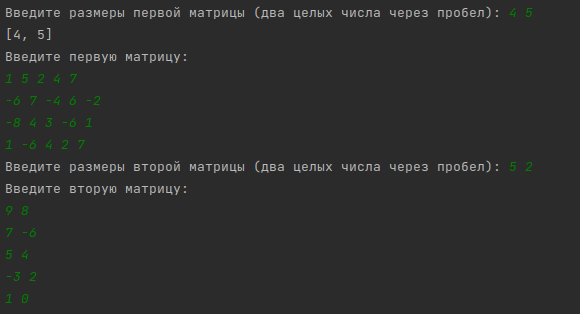
\includegraphics[width=0.7\linewidth]{images/example1}
	\caption{Ввод данных}
	\label{fig:work_example1}
\end{figure}

\begin{figure}[H]
	\centering
	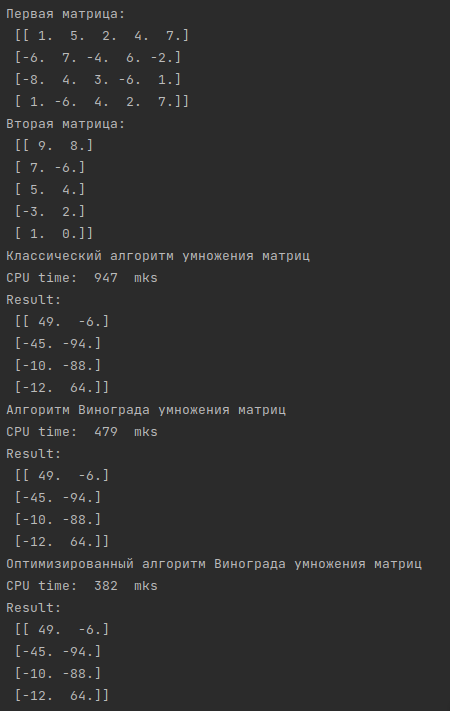
\includegraphics[width=0.7\linewidth]{images/example2}
	\caption{Результат работы программы}
	\label{fig:work_example2}
\end{figure}

\section{Технические характеристики}
Технические характеристики устройства, на котором выполнялось тестирование:
\begin{itemize}
	\item операционная система: Ubuntu 20.01 Linux x86\_64~\cite{ubuntu};
	\item оперативная память: 8 Гб;
	\item процессор: AMD Ryzen5 3500U~\cite{processor}.
\end{itemize}

\section{Время выполнения алгоритмов}

Время выполнения алгоритмов замерялось на автоматически генерируемых квадратных матрицах необходимого размера с использованием функции getrusage библиотеки resources~\cite{resource}. Усредненные результаты замеров процессорного времени приведены в таблице. Используемые обозначения: "Классич."\ - классический алгоритм умножения матриц, "Виноград"\ - алгоритм Копперсмита-Винограда, "Опт.Виноград"\ - оптимизированный алгоритм Копперсмита-Винограда.  

\begin{table}[h]
	\begin{center}
		\captionsetup{justification=raggedleft, singlelinecheck=false}
		\caption{\label{time} Время обработки строк разной длины в микросекундах}
		\begin{tabular}{|c c c c|} 
			\hline
			Размер&Классич.&Виноград&Опт.Виноград\\ [0.5ex]
			\hline
			10 &  7626 &  8432 &  6334\\ 
			\hline
			11 &  10114 &  11119 &  8247\\ 
			\hline
			30 &  198387 &  200491 &  144975\\ 
			\hline
			31 &  221763 &  221463 &  159228\\ 
			\hline
			50 &  914673 &  913305 &  651054\\ 
			\hline
			51 &  990919 &  975478 &  695120\\ 
			\hline
			70 &  2568877 &  2492211 &  1768562\\ 
			\hline
			71 &  2692695 &  2625663 &  1855013\\ 
			\hline
			90 &  5472335 &  5286995 &  3717559\\ 
			\hline
			91 &  5634068 &  5480780 &  3892148\\ 
			\hline
			110 &  10070443 &  9613919 &  6775491\\ 
			\hline
			111 &  10310690 &  9927475 &  7034633\\ 
			\hline
		\end{tabular}
	\end{center}
\end{table}

\begin{figure}[H]
	\centering
	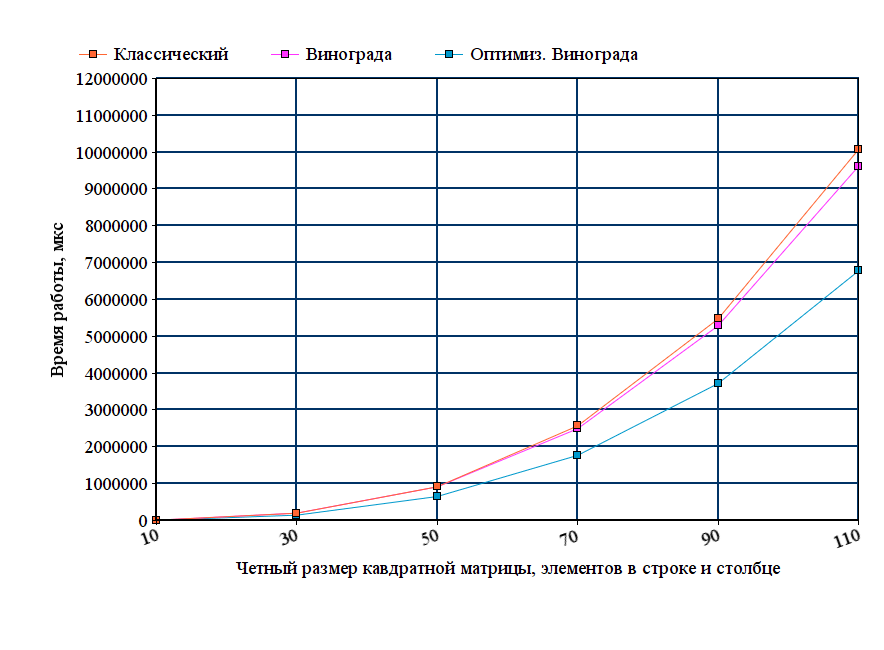
\includegraphics[width=1\linewidth]{images/odd_mat}
	\caption{Сравнение времени работы алгоритмов умножения квадратных матриц четных размеров}
	\label{fig:odd_graph}
\end{figure}

\begin{figure}[H]
	\centering
	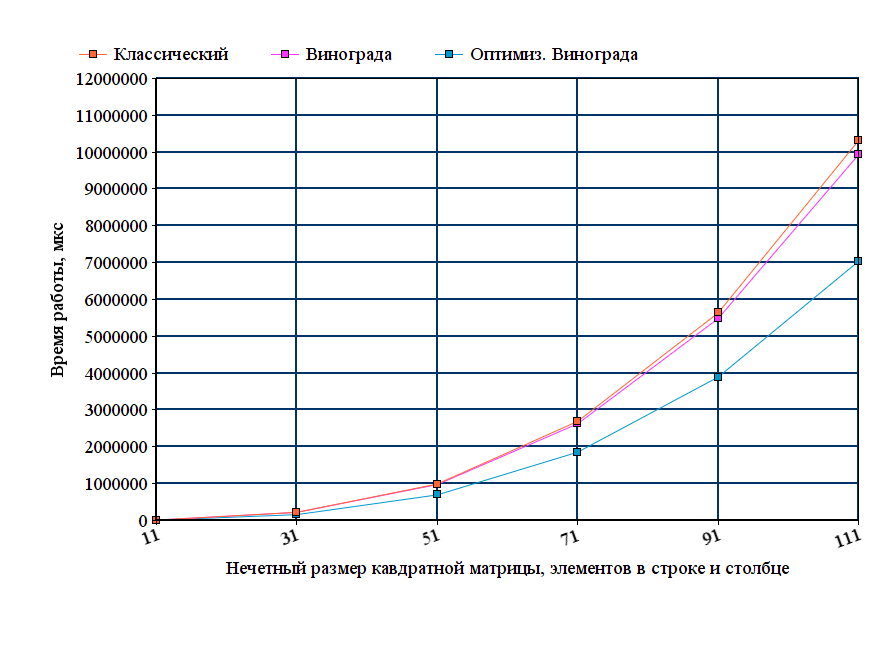
\includegraphics[width=1\linewidth]{images/even_mat}
	\caption{Сравнение времени работы алгоритмов умножения квадратных матриц нечетных размеров}
	\label{fig:even_graph}
\end{figure}

\section{Выводы}

По результатам проведенных замеров видно, что оптимизированный алгоритм Копперсмита-Винограда работает в 1.2-1.5 раза быстрее классического алгоритма умножения матриц с увеличением этого коэффициента при увеличении размера матрицы. Важно заметить, что коэффициент незначительно меньше для матриц нечетных размеров, что говорит о более медленной работе оптимизированного алгоритма Винограда для таких матриц, в то время как классический алгоритм зависимости от четности размеров не имеет. Алгоритм Копперсмита-Винограда на четных матрицах меньше 50x50 работает медленнее классического алгоритма, на больших - чуть быстрее, однако разрыв составляет не более 1.05 раз. В случае с нечетным размером матрицы алгоритм Винограда на небольших матрицах проигрывает классическому алгоритму, но при увеличении размерности время работы обоих алгоритмов сопоставимо, с небольшим преимуществом алгоритма Винограда.
\newpage

\addcontentsline{toc}{chapter}{Заключение}
\chapter*{Заключение}
В процессе выполнения лабораторной работы были изучены и реализованы классический алгоритм умножения и алгоритм Копперсмита-Винограда матриц, оптимизирован алгоритм Винограда.

Согласно проведенному анализу трудоемкости алгоритмов в соответствии с выбранной моделью вычислений, трудоемкость классического алгоритма составила приблизительно $11mnq$, алгоритма Копперсмита-Винограда - $16mnq$, оптимизированного алгоритма Копперсмита-Винограда - $9mnq$.

Было исследовано процессорное время выполнения выше обозначенных алгоритмов. В результате было выявлено, что на матрицах с количеством элементов в строках и столбцах, меньших 50, дольше всего работает алгоритм Копперсмита-Винограда, на больших - классический, причем время работы алгоритма Винограда незначительно меньше (разница не превышает 1.04 раз). Быстрее всего работает оптимизированный алгоритм Копперсмита-Винограда (в 1.2-1.5 раз быстрее других алгоритмов с увеличением разницы во времени работы с увеличением размеров матриц), однако заметна небольшая деградация времени работы для матриц с нечетным количеством строк и столбцов (как и у алгоритма Винограда-Копперсмита), тогда как классический алгоритм таким свойством не обладает.

\newpage
\addcontentsline{toc}{chapter}{Список литературы}

\bibliographystyle{utf8gost705u}
\bibliography{bib_lab_2}
\nocite{*}



\end{document}